\documentclass[11pt,a4paper]{article}

% ── Encoding & Language ──────────────────────────────────────────────────────
\usepackage[utf8]{inputenc}
\usepackage[T1]{fontenc}
\usepackage[english]{babel}

% ── Page geometry ────────────────────────────────────────────────────────────
\usepackage[top=2.5cm, bottom=2.5cm, left=2.8cm, right=2.8cm]{geometry}

% ── Fonts ────────────────────────────────────────────────────────────────────
\usepackage{lmodern}
\usepackage{microtype}

% ── Math ─────────────────────────────────────────────────────────────────────
\usepackage{amsmath, amssymb, amsthm}
\usepackage{mathtools}
\theoremstyle{definition}
\newtheorem{theorem}{Theorem}
\newtheorem{definition}{Definition}
\newtheorem{remark}{Remark}

% ── Graphics & Figures ───────────────────────────────────────────────────────
\usepackage{graphicx}
\usepackage{float}
\usepackage{caption}
\usepackage{subcaption}
\graphicspath{{output/}}

% ── Tables ───────────────────────────────────────────────────────────────────
\usepackage{booktabs}
\usepackage{array}
\usepackage{tabularx}

% ── Code listings ────────────────────────────────────────────────────────────
\usepackage{listings}
\usepackage{xcolor}

\definecolor{codebg}{rgb}{0.97,0.97,0.97}
\definecolor{codegreen}{rgb}{0.0,0.5,0.0}
\definecolor{codekw}{rgb}{0.13,0.13,0.7}
\definecolor{codestring}{rgb}{0.7,0.1,0.1}
\definecolor{codecomment}{rgb}{0.4,0.4,0.4}

\lstset{
  language=Python,
  backgroundcolor=\color{codebg},
  basicstyle=\footnotesize\ttfamily,
  keywordstyle=\color{codekw}\bfseries,
  stringstyle=\color{codestring},
  commentstyle=\color{codecomment}\itshape,
  numberstyle=\tiny\color{gray},
  numbers=left,
  stepnumber=1,
  numbersep=8pt,
  frame=single,
  framerule=0.4pt,
  rulecolor=\color{gray!40},
  breaklines=true,
  breakatwhitespace=true,
  showstringspaces=false,
  tabsize=4,
  captionpos=b,
}

% ── Hyperlinks ───────────────────────────────────────────────────────────────
\usepackage[colorlinks=true, linkcolor=blue!70!black, urlcolor=blue!70!black, citecolor=green!50!black]{hyperref}

% ── Headers & Footers ────────────────────────────────────────────────────────
\usepackage{fancyhdr}
\pagestyle{fancy}
\fancyhf{}
\lhead{\small SVD \& PCA for Medical Image Analysis}
\rhead{\small Statistical Methods --- Politecnico di Bari}
\cfoot{\thepage}
\renewcommand{\headrulewidth}{0.4pt}

% ── Misc ─────────────────────────────────────────────────────────────────────
\usepackage{enumitem}
\usepackage{tocloft}
\usepackage[export]{adjustbox}
\renewcommand{\cftsecleader}{\cftdotfill{\cftdotsep}}

% ─────────────────────────────────────────────────────────────────────────────
\begin{document}

% ═══════════════════════════════════ TITLE PAGE ═══════════════════════════════
\begin{titlepage}
  \centering
  \vspace*{1.5cm}

  {\Large\scshape Politecnico di Bari\\[6pt]
  Department of Electrical and Information Engineering (DEI)}

  \vspace{1cm}
  \rule{\linewidth}{1.2pt}\\[8pt]
  {\Huge\bfseries SVD or PCA for\\[6pt] Image Analysis in\\[6pt] Medical Diagnostics}\\[8pt]
  \rule{\linewidth}{1.2pt}

  \vspace{1.5cm}
  {\large\itshape Statistical Methods --- Project Report}\\[0.4cm]
  {\large Academic Year 2025/2026 --- 1st Year, 1st Semester}

  \vspace{1.5cm}
  \begin{tabular}{ll}
    \textbf{Student:}  & Andrea Patruno \\[4pt]
    \textbf{Course:}   & Statistical Methods for Machine Learning \\[4pt]
    \textbf{Dataset:}  & Lung X-Rays Grayscale (4 diagnostic classes) \\[4pt]
    \textbf{Language:} & Python 3.12 \\
  \end{tabular}

  \vfill
  {\small\today}
\end{titlepage}

% ═══════════════════════════════ TABLE OF CONTENTS ═══════════════════════════
\tableofcontents
\newpage

% ═══════════════════════════════ SECTION 1 ═══════════════════════════════════
\section{Problem Description and Motivation}

\subsection{Clinical Motivation}

Chest X-rays are among the most widely used diagnostic tools in modern medicine.
Every hospital produces thousands of radiographic images per day, creating two
concrete engineering challenges:

\begin{enumerate}[nosep]
  \item \textbf{Storage.} A high-resolution radiograph can occupy tens of MB.
        At hospital scale, efficient compression without diagnostic loss is critical.
  \item \textbf{Telemedicine transmission.} Remote diagnostics requires sending
        images over bandwidth-limited networks, demanding lightweight yet
        faithful representations.
\end{enumerate}

This project addresses two research questions:

\begin{enumerate}[nosep]
  \item Can Singular Value Decomposition compress chest X-rays while preserving
        diagnostically relevant information?
  \item Can Principal Component Analysis reveal latent structure in the dataset
        that distinguishes different pulmonary pathologies?
\end{enumerate}

\subsection{Dataset}

The dataset consists of grayscale chest X-rays divided into \textbf{four
diagnostic classes}:

\begin{table}[H]
\centering
\begin{tabularx}{0.9\textwidth}{llcc}
\toprule
\textbf{Class} & \textbf{Pathology} & \textbf{Available} & \textbf{Used} \\
\midrule
Corona Virus Disease & COVID-19 pneumonia    & 122 & $\leq 80$ \\
Normal               & Healthy lungs         & 540 & $\leq 80$ \\
Pneumonia            & Bacterial/viral pneu. & 186 & $\leq 80$ \\
Tuberculosis         & Pulmonary tuberculosis& 333 & $\leq 80$ \\
\bottomrule
\end{tabularx}
\caption{Dataset composition. Images are capped at 80 per class to balance computation time.}
\end{table}

\begin{remark}[Imbalanced dataset]
  The classes have very different cardinalities: Normal contains $\approx 4\times$
  more images than COVID-19. This imbalance can bias PCA components toward the
  Normal class patterns. Comparative conclusions should be interpreted with this
  limitation in mind.
\end{remark}

Raw images have heterogeneous resolutions (from $203\times230$ px for COVID-19 to
$1\,654\times1\,678$ px for Normal). Each image is uniformly resized to
$256\times256$ px using Lanczos interpolation before analysis.

\subsubsection*{Histogram observations (Exploration Phase)}

\begin{itemize}[nosep]
  \item \textbf{COVID-19:} intensity concentrated in mid-high range (100--170), consistent with ground-glass opacities.
  \item \textbf{Normal:} uniform distribution across the full range, good tissue contrast.
  \item \textbf{Pneumonia:} strong peak in dark tones (30--80), consistent with dense pulmonary consolidations.
  \item \textbf{Tuberculosis:} bimodal distribution with peak in bright tones (150--190), indicative of fibrotic/calcified lesions.
\end{itemize}

\begin{figure}[H]
  \centering
  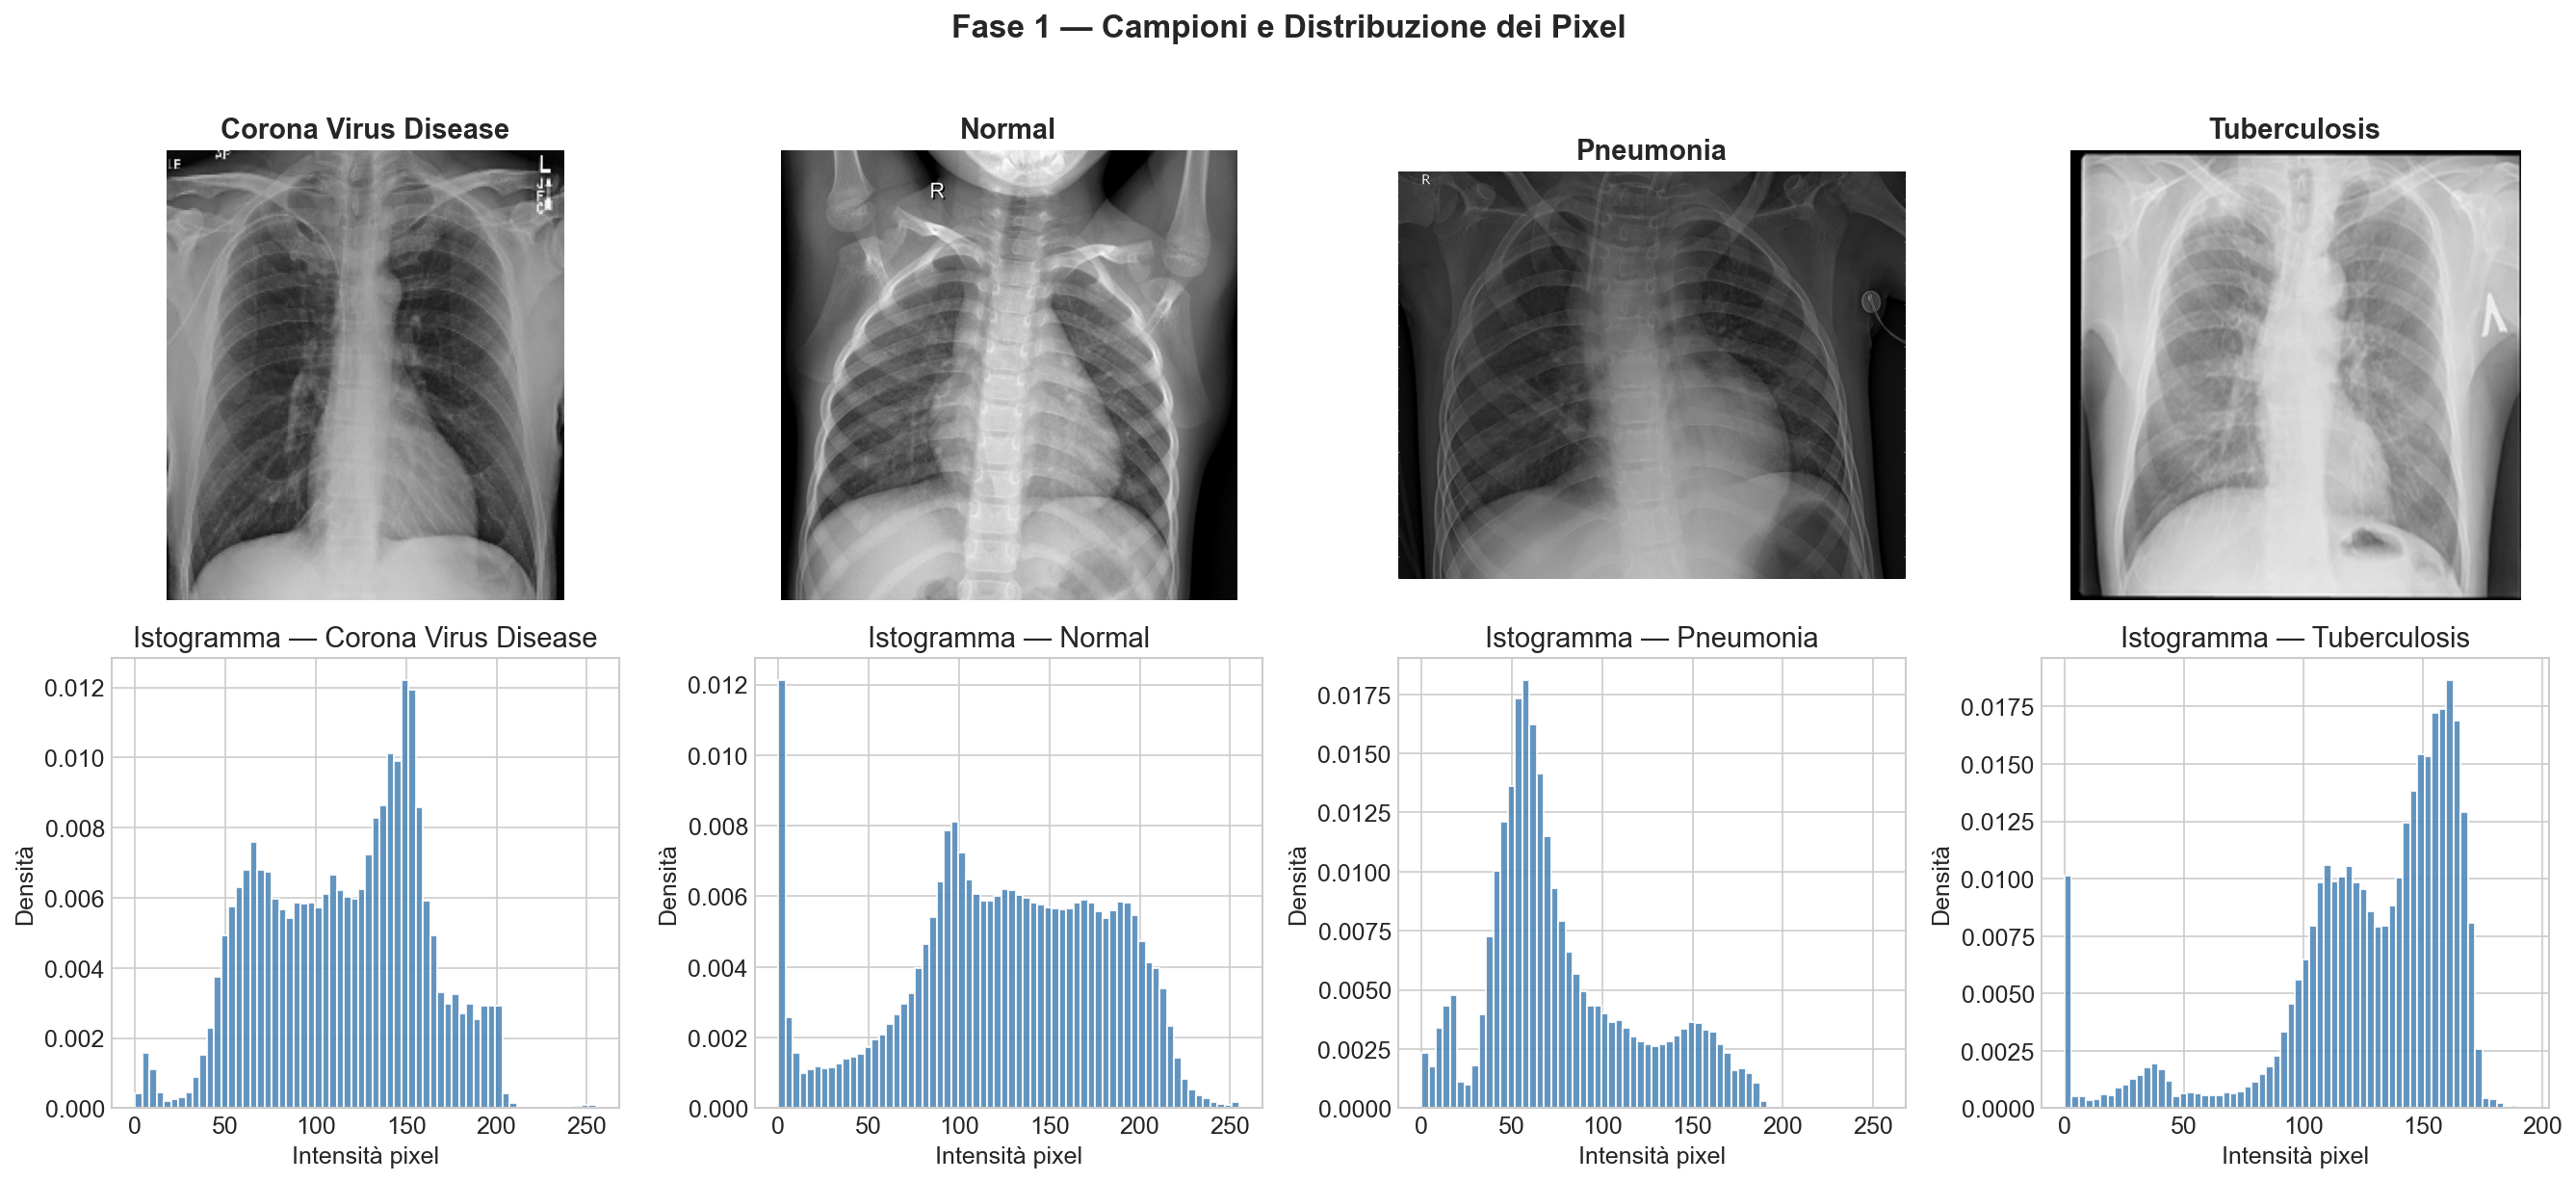
\includegraphics[width=\linewidth]{fase1_esplorazione.png}
  \caption{Phase 1 --- Sample radiographs and pixel intensity histograms for each class.}
\end{figure}


% ═══════════════════════════════ SECTION 2 ═══════════════════════════════════
\section{Theoretical Background}

\subsection{Singular Value Decomposition (SVD)}

\begin{definition}[SVD]
  For any matrix $A \in \mathbb{R}^{m \times n}$, there exist orthogonal matrices
  $U \in \mathbb{R}^{m \times m}$, $V \in \mathbb{R}^{n \times n}$, and a
  non-negative diagonal matrix $\Sigma \in \mathbb{R}^{m \times n}$ such that
  \[
    A = U \Sigma V^T,
  \]
  where the diagonal entries $\sigma_1 \geq \sigma_2 \geq \cdots \geq \sigma_r \geq 0$
  (with $r = \min(m,n)$) are the \emph{singular values} of $A$.
\end{definition}

\noindent The columns of $U$ are called \emph{left singular vectors} (capture row-wise spatial
structure), while the rows of $V^T$ are \emph{right singular vectors} (capture column-wise
structure). The singular values quantify the ``importance'' of each component:
$\sigma_1$ encodes the direction of highest energy variation, and subsequent values
capture progressively finer patterns.

\medskip
\noindent\textbf{connection with eigendecomposition.}
The singular values and vectors satisfy:
\[
  A^T A \,v_i = \sigma_i^2\, v_i, \qquad
  A A^T \,u_i = \sigma_i^2\, u_i,
\]
so the columns of $V$ are eigenvectors of $A^TA$ and the columns of $U$ are
eigenvectors of $AA^T$, with $\sigma_i = \sqrt{\lambda_i}$.

\subsubsection{Rank-$k$ Approximation}

Retaining only the first $k$ components yields the \emph{truncated SVD}
(also called economy SVD when $k = r$):
\[
  A_k = \sum_{i=1}^{k} \sigma_i\, \mathbf{u}_i\, \mathbf{v}_i^T
        = U_k\, \Sigma_k\, V_k^T.
\]

\begin{theorem}[Eckart--Young, 1936]
  Among all matrices of rank at most $k$, $A_k$ is the closest to $A$ in both
  the spectral norm and the Frobenius norm:
  \[
    A_k = \underset{\operatorname{rank}(B)\,\leq\,k}{\arg\min}\;\|A - B\|_F,
  \]
  with minimum error
  \[
    \|A - A_k\|_F = \sqrt{\sum_{i=k+1}^{r} \sigma_i^2},
    \qquad
    \|A - A_k\|_2 = \sigma_{k+1}.
  \]
\end{theorem}

\noindent This theorem provides the theoretical optimality guarantee for SVD-based
image compression: \emph{no other rank-$k$ decomposition can approximate the
original image more faithfully}.

\subsubsection{Compression Ratio and Quality Metrics}

With $k$ components, one stores $k(m+n+1)$ values instead of $mn$:
\[
  \text{compression ratio} = \frac{k(m+n+1)}{mn}.
\]
For $m = n = 256$ and $k = 20$: compression ratio $\approx 15.7\%$.

\medskip
\noindent Two standard metrics evaluate reconstruction quality:

\begin{center}
\begin{tabularx}{0.88\textwidth}{lXl}
\toprule
\textbf{Metric} & \textbf{Formula} & \textbf{Threshold (radiology)}\\
\midrule
MSE  & $\dfrac{1}{mn}\displaystyle\sum_{i,j}(A_{ij}-\hat A_{ij})^2$ & lower is better \\[8pt]
PSNR & $10\log_{10}\!\left(\dfrac{1}{\text{MSE}}\right)$ [dB]       & $>30$ dB acceptable \\
\bottomrule
\end{tabularx}
\end{center}

\begin{remark}
  Pixel-wise metrics (MSE, PSNR) do not directly capture clinical saliency.
  A reconstructed image may score PSNR $>30$ dB yet exhibit subtle artefacts
  in diagnostically critical regions (e.g., lesion boundaries). They are
  nonetheless the engineering standard for compression fidelity assessment.
\end{remark}

\subsubsection{Efficient MSE Computation}

By the Eckart--Young theorem, the MSE at rank $k$ can be computed directly from
the singular values, without reconstructing the image:
\[
  \mathrm{MSE}(k)
    = \frac{\|A - A_k\|_F^2}{mn}
    = \frac{\displaystyle\sum_{i=k+1}^{r}\sigma_i^2}{mn}.
\]
This avoids 200 full matrix multiplications when computing the MSE curve over
$k = 1, \ldots, 200$.

% ─────────────────────────────────────────────────────────────────────────────
\subsection{Principal Component Analysis (PCA)}

\begin{definition}[PCA]
  Given a data matrix $X \in \mathbb{R}^{N \times d}$ (each row is an
  observation), PCA finds an ordered orthonormal basis
  $\{v_1, v_2, \ldots, v_k\}$ such that the projection
  $X_{\text{PCA}} = X V_k$ has maximum variance in each successive direction.
\end{definition}

\noindent The standard algorithm proceeds as follows:

\begin{enumerate}[nosep]
  \item \textbf{Flatten.} Each image $(256\times256)$ is unrolled into a vector $\mathbf{x}\in\mathbb{R}^{65536}$.
  \item \textbf{Stack.} Form data matrix $X \in \mathbb{R}^{N \times 65536}$.
  \item \textbf{Center.} Subtract the column mean: $\tilde X = X - \bar X$.
  \item \textbf{PCA.} Find the top-$k$ eigenvectors of the covariance matrix
        $C = \tfrac{1}{N-1}\tilde X^T \tilde X \in \mathbb{R}^{d \times d}$.
  \item \textbf{Project.} $X_{\text{PCA}} = \tilde X\, V_k \in \mathbb{R}^{N \times k}$.
\end{enumerate}

\subsubsection{Choosing $k$: Percentage of Variance Explained}

The $i$-th principal component explains a fraction
$\lambda_i / \sum_j \lambda_j$ of the total variance.
In practice, $k$ is chosen via a \emph{scree plot} (elbow method) or by
requiring a cumulative explained variance threshold (e.g., 90\% or 95\%).

\subsubsection{Eigenfaces / Eigen-X-rays}

The eigenvectors $v_i$ of $C$ can be reshaped and visualised as
$256\times 256$ images. In the context of chest X-rays they encode the dominant
modes of visual variability across the dataset (global contrast, lateral
symmetry, mediastinal structure, etc.).

% ─────────────────────────────────────────────────────────────────────────────
\subsection{Relationship between SVD and PCA}
\label{sec:svd-pca}

A crucial theoretical insight is that \textbf{PCA is equivalent to the SVD of
the centred data matrix}:

\[
  \tilde X = U\,\Sigma\, V^T
  \quad\Longrightarrow\quad
  C = \tfrac{1}{N-1}\tilde X^T \tilde X
    = \tfrac{1}{N-1} V\Sigma^2 V^T.
\]

Hence the columns of $V$ are simultaneously the right singular vectors of
$\tilde X$ and the eigenvectors of $C$, with eigenvalues
$\lambda_i = \sigma_i^2/(N-1)$.

\medskip
\begin{center}
\begin{tabularx}{0.9\textwidth}{lXX}
\toprule
& \textbf{SVD for compression} & \textbf{PCA for analysis} \\
\midrule
Input  & Single image $A \in \mathbb{R}^{m\times n}$ & Dataset $X \in \mathbb{R}^{N\times d}$ \\
Output & Approximation $A_k$ & Projection $X_\text{PCA} \in \mathbb{R}^{N\times k}$ \\
Goal   & Reduce storage footprint & Find shared latent structure \\
Theoretical guarantee & Eckart--Young optimality & Maximum variance directions \\
Use case & Compression, transmission & Visualisation, clustering \\
\bottomrule
\end{tabularx}
\end{center}

\medskip
\noindent SVD and PCA are \textbf{complementary}, not alternatives.
The SVD is applied \emph{per image} to compress it; the PCA is applied to the
\emph{entire dataset} to reveal its collective structure.


% ═══════════════════════════════ SECTION 3 ═══════════════════════════════════
\section{Implementation}

\subsection{Software Architecture}

The project is written in Python~3.12 and organised into independent modules
following the Single Responsibility Principle:

\begin{lstlisting}[caption={Project structure}]
Medical Image Compression and Analysis/
|-- config.py          # global parameters (paths, constants, plot style)
|-- data_loader.py     # loading, validation, tilt correction  (Phases 1-2)
|-- svd_engine.py      # SVD, truncated reconstruction, MSE/PSNR (Phase 3)
|-- visualization.py   # plots for phases 1, 2, 4
|-- src/analysis.py    # scree plot, MSE/PSNR curves, PCA, eigenfaces (Phase 5)
|-- main.py            # orchestration script
|-- medical_image_svd_pca.ipynb   # interactive notebook
`-- output/            # saved figures (.png, 150 dpi)
\end{lstlisting}

\noindent Core dependencies: \texttt{numpy}, \texttt{scipy}, \texttt{Pillow},
\texttt{scikit-learn}, \texttt{matplotlib}, \texttt{seaborn}.

\subsection{Key Configurable Parameters}

\begin{table}[H]
\centering
\begin{tabular}{llp{6cm}}
\toprule
\textbf{Parameter} & \textbf{Default} & \textbf{Description} \\
\midrule
\texttt{TARGET\_SIZE}     & \texttt{(256, 256)} & Resize resolution \\
\texttt{MAX\_PER\_CLASS}  & \texttt{80}         & Images per class \\
\texttt{CORRECT\_TILT}    & \texttt{True}       & Enable tilt correction \\
\texttt{MAX\_TILT\_ANGLE} & \texttt{10}         & Max allowed tilt (degrees) \\
\texttt{K\_VALUES\_DEMO}  & \texttt{[1,5,10,20,50,100,200]} & $k$ values for Phase 4 \\
\texttt{K\_RANGE\_METRICS}& \texttt{range(1, 201)} & $k$ range for MSE/PSNR curves \\
\texttt{PCA\_N\_COMPONENTS} & \texttt{50}       & Number of PCA components \\
\bottomrule
\end{tabular}
\caption{Global parameters defined in \texttt{config.py}.}
\end{table}

\subsection{Phase 2 --- Pre-processing Pipeline}

\begin{lstlisting}[caption={Core pre-processing pipeline in \texttt{data\_loader.py}}]
# 1. Load as grayscale
img = Image.open(path).convert('L')

# 2. Resize to 256x256 with Lanczos interpolation
img = img.resize((256, 256), Image.LANCZOS)
arr = np.array(img, dtype=np.float64) / 255.0  # normalise [0,1]

# 3. Detect and correct tilt
if apply_tilt_correction:
    arr, angle = correct_tilt(arr, angle=angle)
    arr = np.clip(arr, 0, 1)
\end{lstlisting}

\subsubsection*{Tilt Detection Algorithm}

Chest X-rays often exhibit slight rotational misalignment. The detection
algorithm maximises the variance of the gradient of the horizontal projection:
\[
  \theta^* = \arg\max_\theta \operatorname{Var}\!\left(
    \nabla_{\text{row}}\bigl[\operatorname{rotate}(A,\,-\theta)\bigr]
  \right).
\]
A two-pass search is used for efficiency: a coarse scan (step $2^\circ$,
range $\pm 25^\circ$) on a thumbnail image ($128\,\mathrm{px}$), followed
by a fine scan (step $0.5^\circ$, window $\pm 3^\circ$ around the coarse best).

Images are discarded if $|\theta^*| > 10^\circ$ (excessive tilt), if they
contain artificial white-padding corners (median brightness $> 130/255$ in three
or more corners), or if they are identified as lateral projections (fewer than
60\% of columns carry significant signal).

\begin{figure}[H]
  \centering
  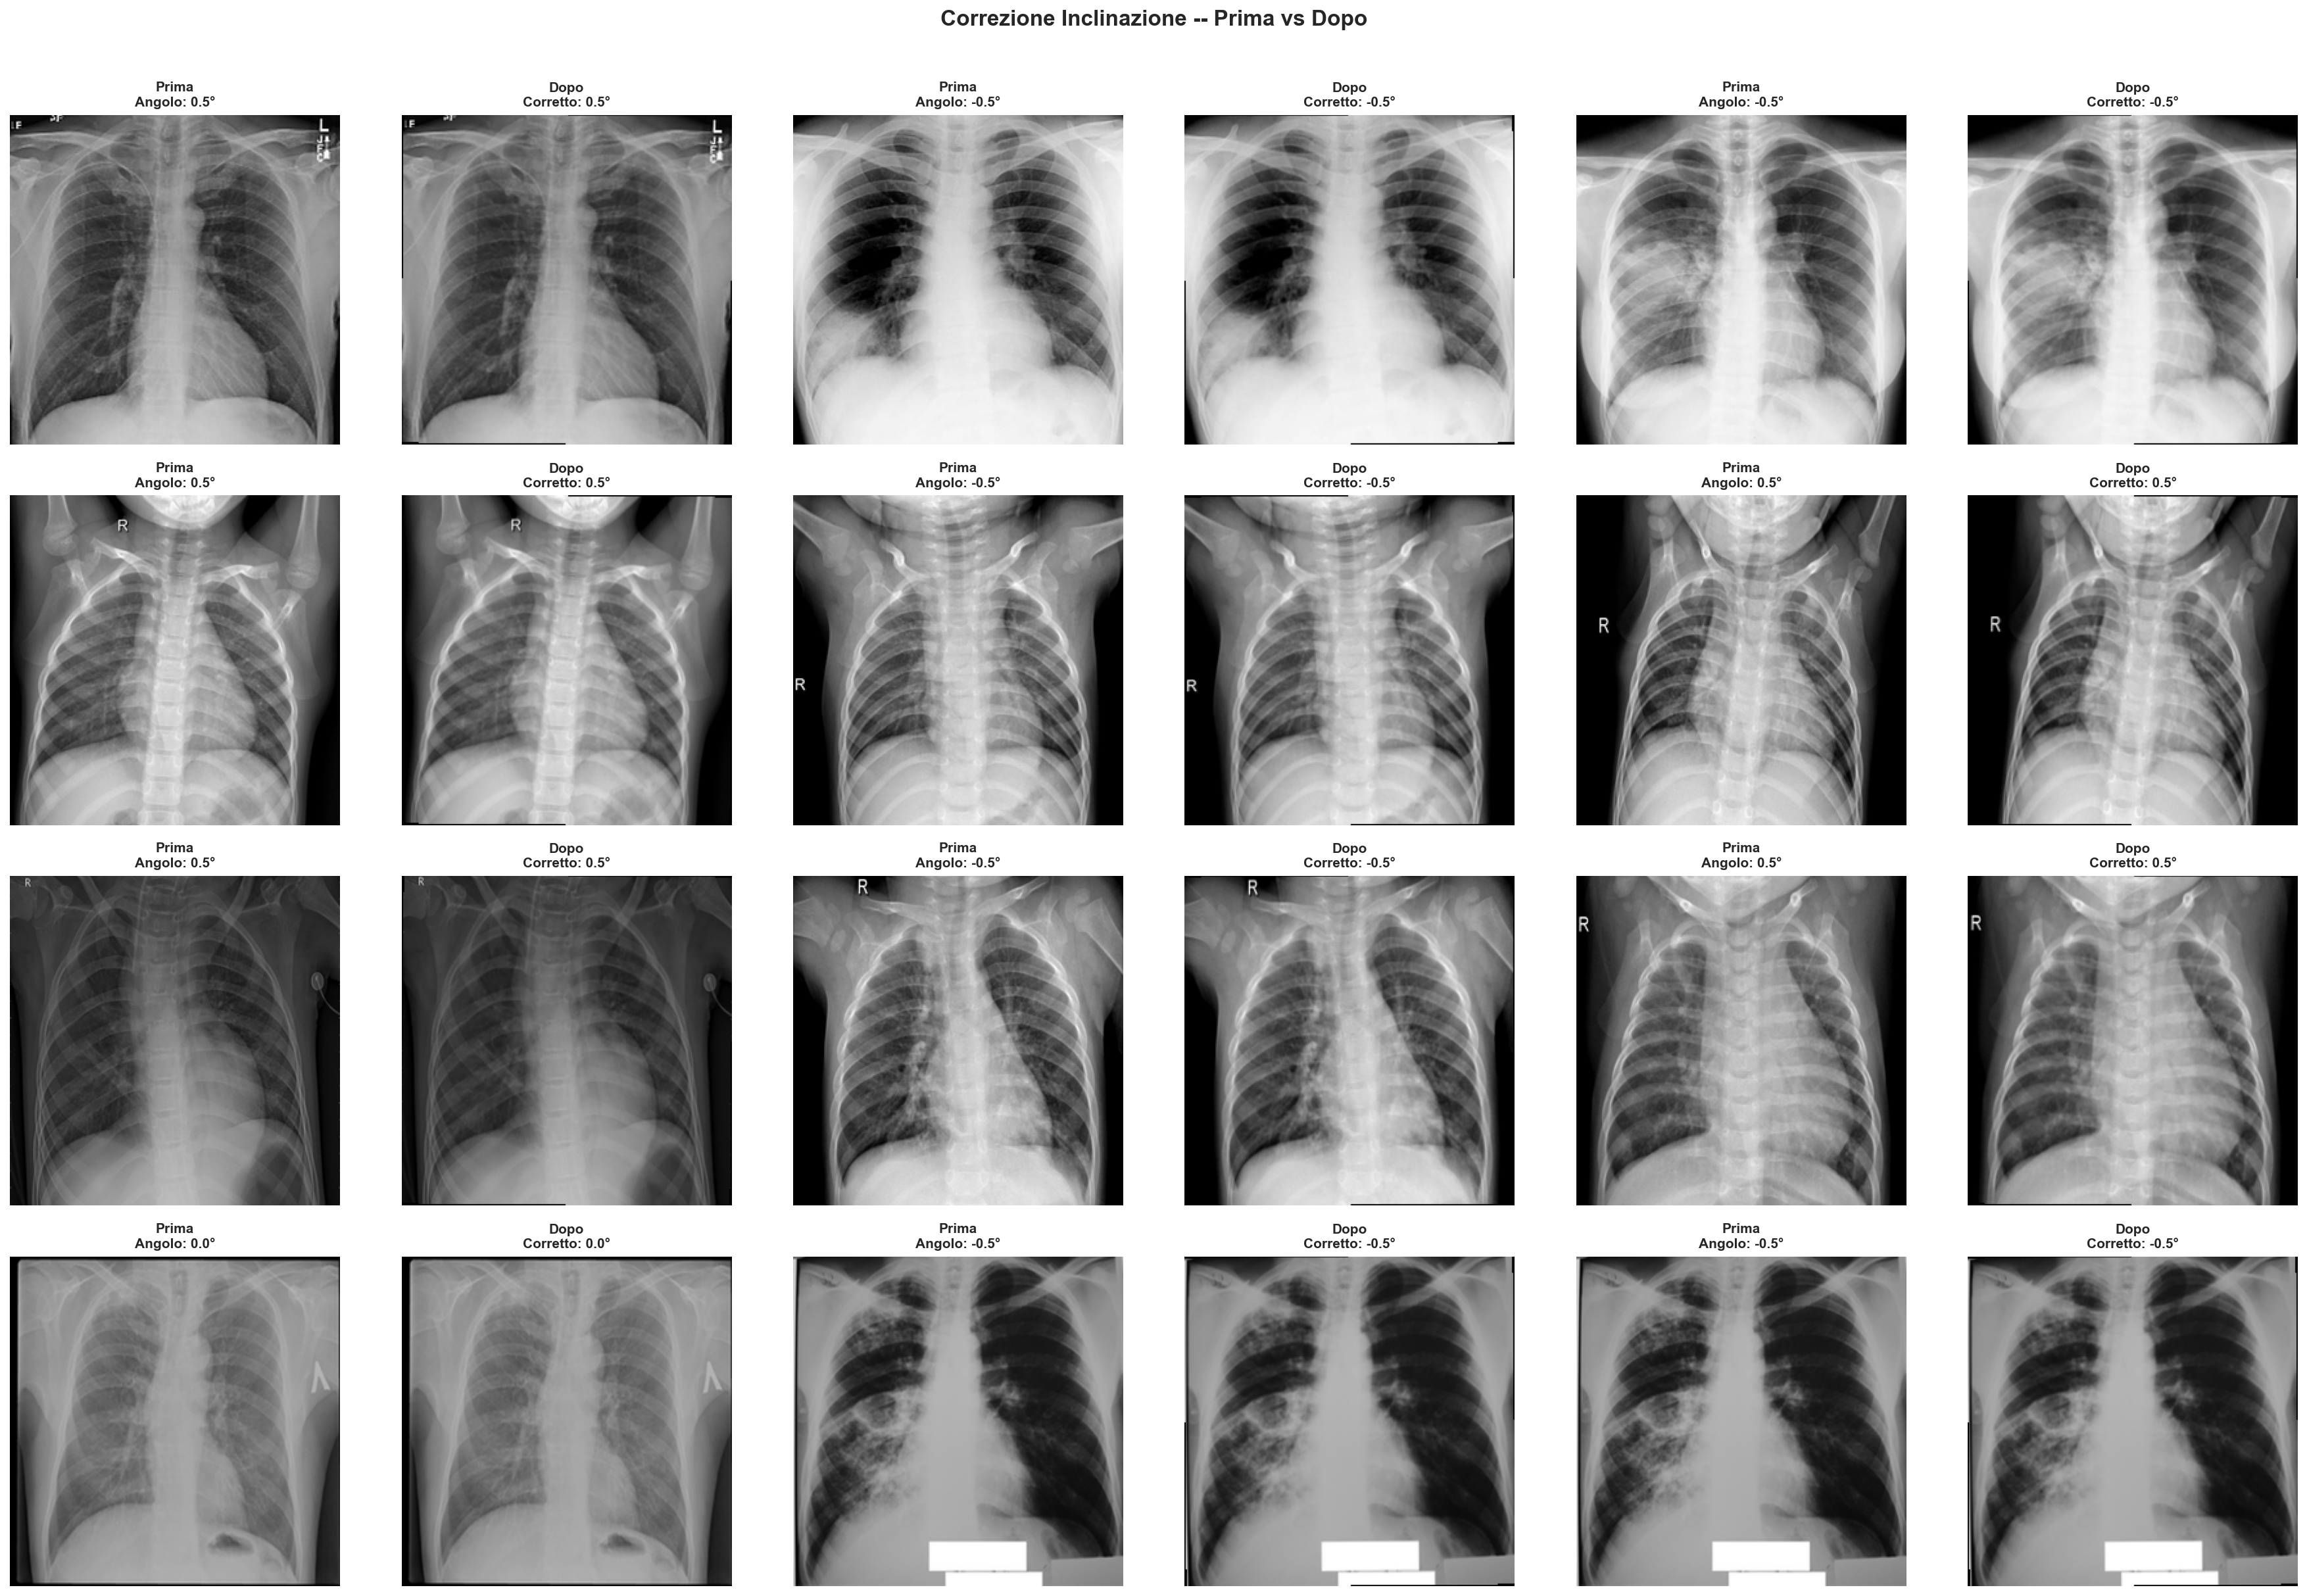
\includegraphics[width=\linewidth]{fase2_correzione_tilt.png}
  \caption{Phase 2 --- Examples of tilt detection and correction.}
\end{figure}

\subsection{Phase 3 --- SVD Engine}

\begin{lstlisting}[caption={SVD core functions in \texttt{svd\_engine.py}}]
import numpy as np

def apply_svd(image_matrix):
    """Economy SVD of a 2-D image array."""
    U, S, Vt = np.linalg.svd(image_matrix, full_matrices=False)
    return U, S, Vt

def reconstruct_svd(U, S, Vt, k):
    """Rank-k reconstruction:  A_k = U_k * diag(S_k) * Vt_k."""
    return (U[:, :k] * S[:k]) @ Vt[:k, :]

def compression_ratio(m, n, k):
    """Fraction of values stored relative to the full image."""
    return min(1.0, k * (m + n + 1) / (m * n))
\end{lstlisting}

\subsection{Phase 5 --- PCA}

\begin{lstlisting}[caption={PCA execution in \texttt{src/analysis.py}}]
from sklearn.decomposition import PCA

def run_pca(all_images, n_components=50):
    X = all_images.reshape(all_images.shape[0], -1)   # (N, 65536)
    pca_model = PCA(n_components=n_components)
    X_pca = pca_model.fit_transform(X)                 # (N, 50)
    return pca_model, X_pca
\end{lstlisting}

\noindent \texttt{sklearn}'s \texttt{PCA} uses a randomised SVD internally
(\texttt{svd\_solver='auto'}), making it numerically stable and efficient even
for high-dimensional inputs like $65536$-feature image vectors.


% ═══════════════════════════════ SECTION 4 ═══════════════════════════════════
\section{Numerical Experiments and Results}

\subsection{Phase 3 --- SVD Decomposition Analysis}

For a $256\times 256$ image (economy SVD), the decomposition produces
$r = 256$ singular values. Key observations:
\begin{itemize}[nosep]
  \item The \emph{first} singular value $\sigma_1 \approx 130$, capturing global
        brightness.
  \item Singular values decay rapidly: after the first 10--15, values are near
        zero.
  \item 90\% of cumulative variance is captured by approximately $k = 1$--$3$
        components.
\end{itemize}

\subsection{Phase 4 --- Reconstruction Quality vs. Rank $k$}

\begin{table}[H]
\centering
\begin{tabular}{rrrll}
\toprule
$k$ & \textbf{Compr. Ratio} & \textbf{PSNR (dB)} & \textbf{Visual quality} \\
\midrule
1   & 0.8\%  & 17.3 & Mean brightness only \\
5   & 3.9\%  & 23.8 & Chest silhouette barely visible \\
10  & 7.8\%  & 27.8 & Ribs, mediastinum beginning to appear \\
\textbf{20}  & \textbf{15.7\%} & \textbf{32.4} & \textbf{Diagnostic quality (PSNR $>30$ dB)} \\
50  & 39.1\% & 40.1 & Diagnostic detail fully preserved \\
100 & 78.3\% & 50.0 & Nearly indistinguishable from original \\
200 & 100\%  & 71.5 & Virtually perfect reconstruction \\
\bottomrule
\end{tabular}
\caption{SVD reconstruction quality as a function of rank $k$
         (256$\times$256 Normal class sample, pixel values in [0,1]).}
\end{table}

\begin{figure}[H]
  \centering
  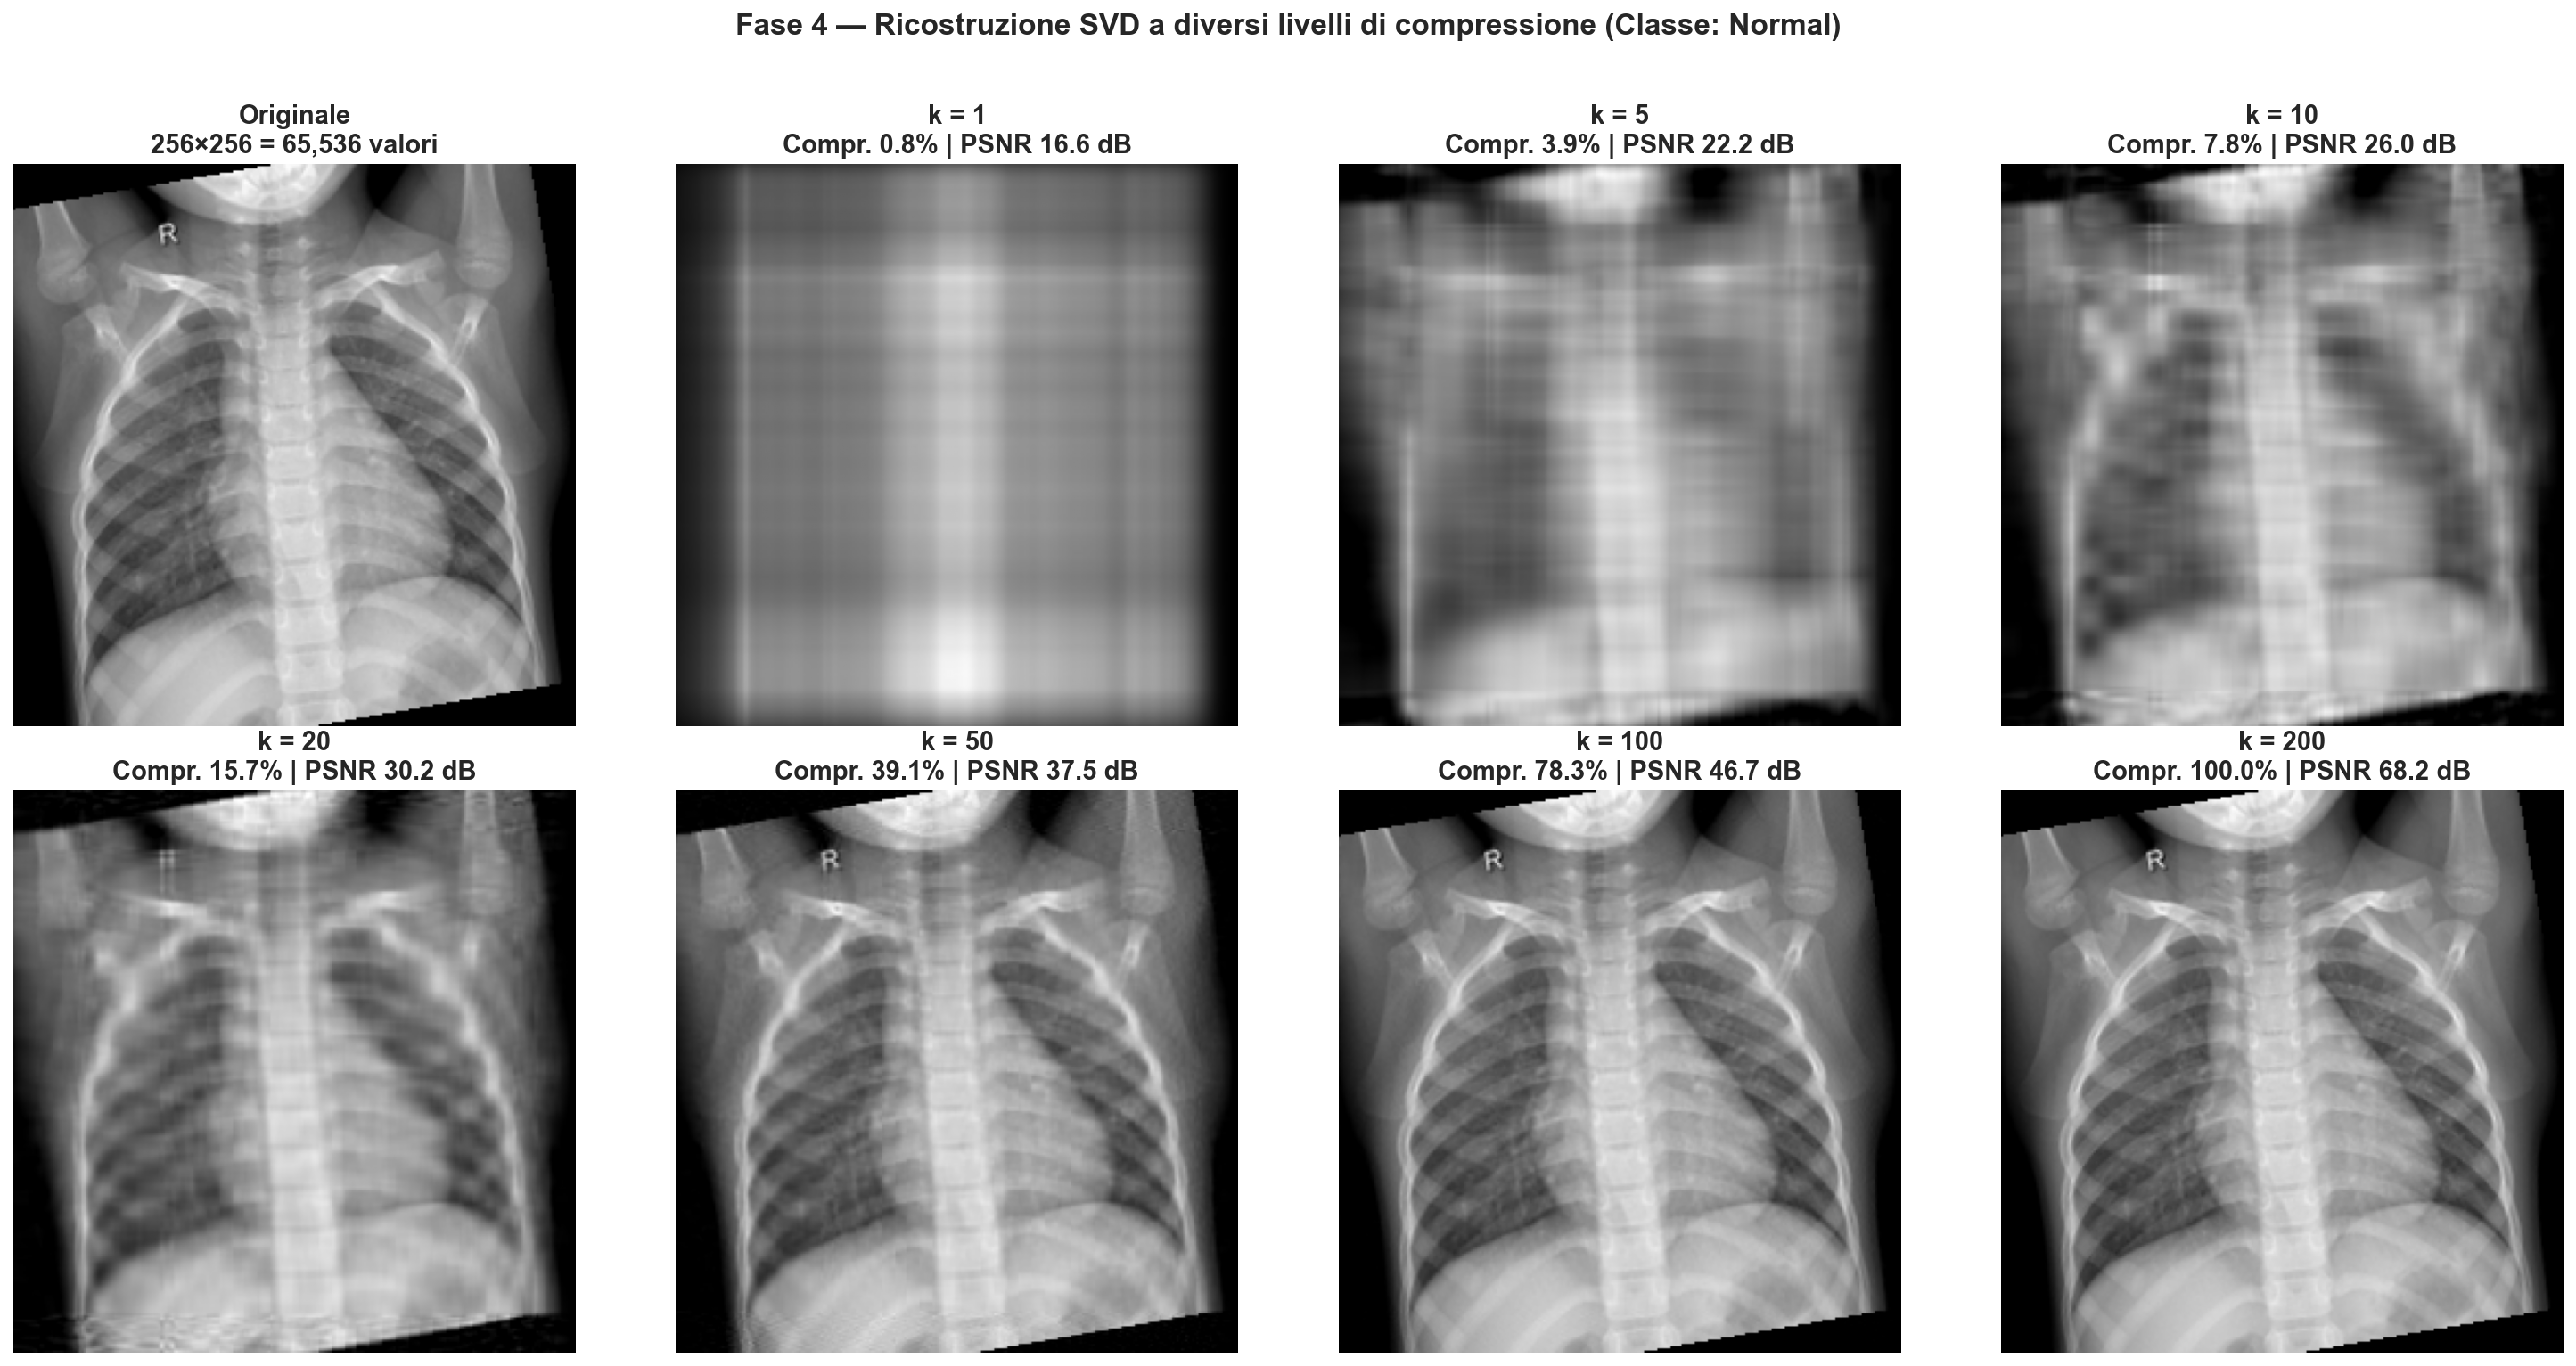
\includegraphics[width=\linewidth]{fase4_ricostruzione_svd.png}
  \caption{Phase 4 --- SVD reconstructions at increasing values of $k$.}
\end{figure}

\noindent\textbf{Key result:} with only $k=20$ components (15.7\% of the
original data), the PSNR exceeds \textbf{32 dB} --- the conventional threshold
for acceptable diagnostic image quality.

\subsubsection*{Inter-class comparison}

\begin{figure}[H]
  \centering
  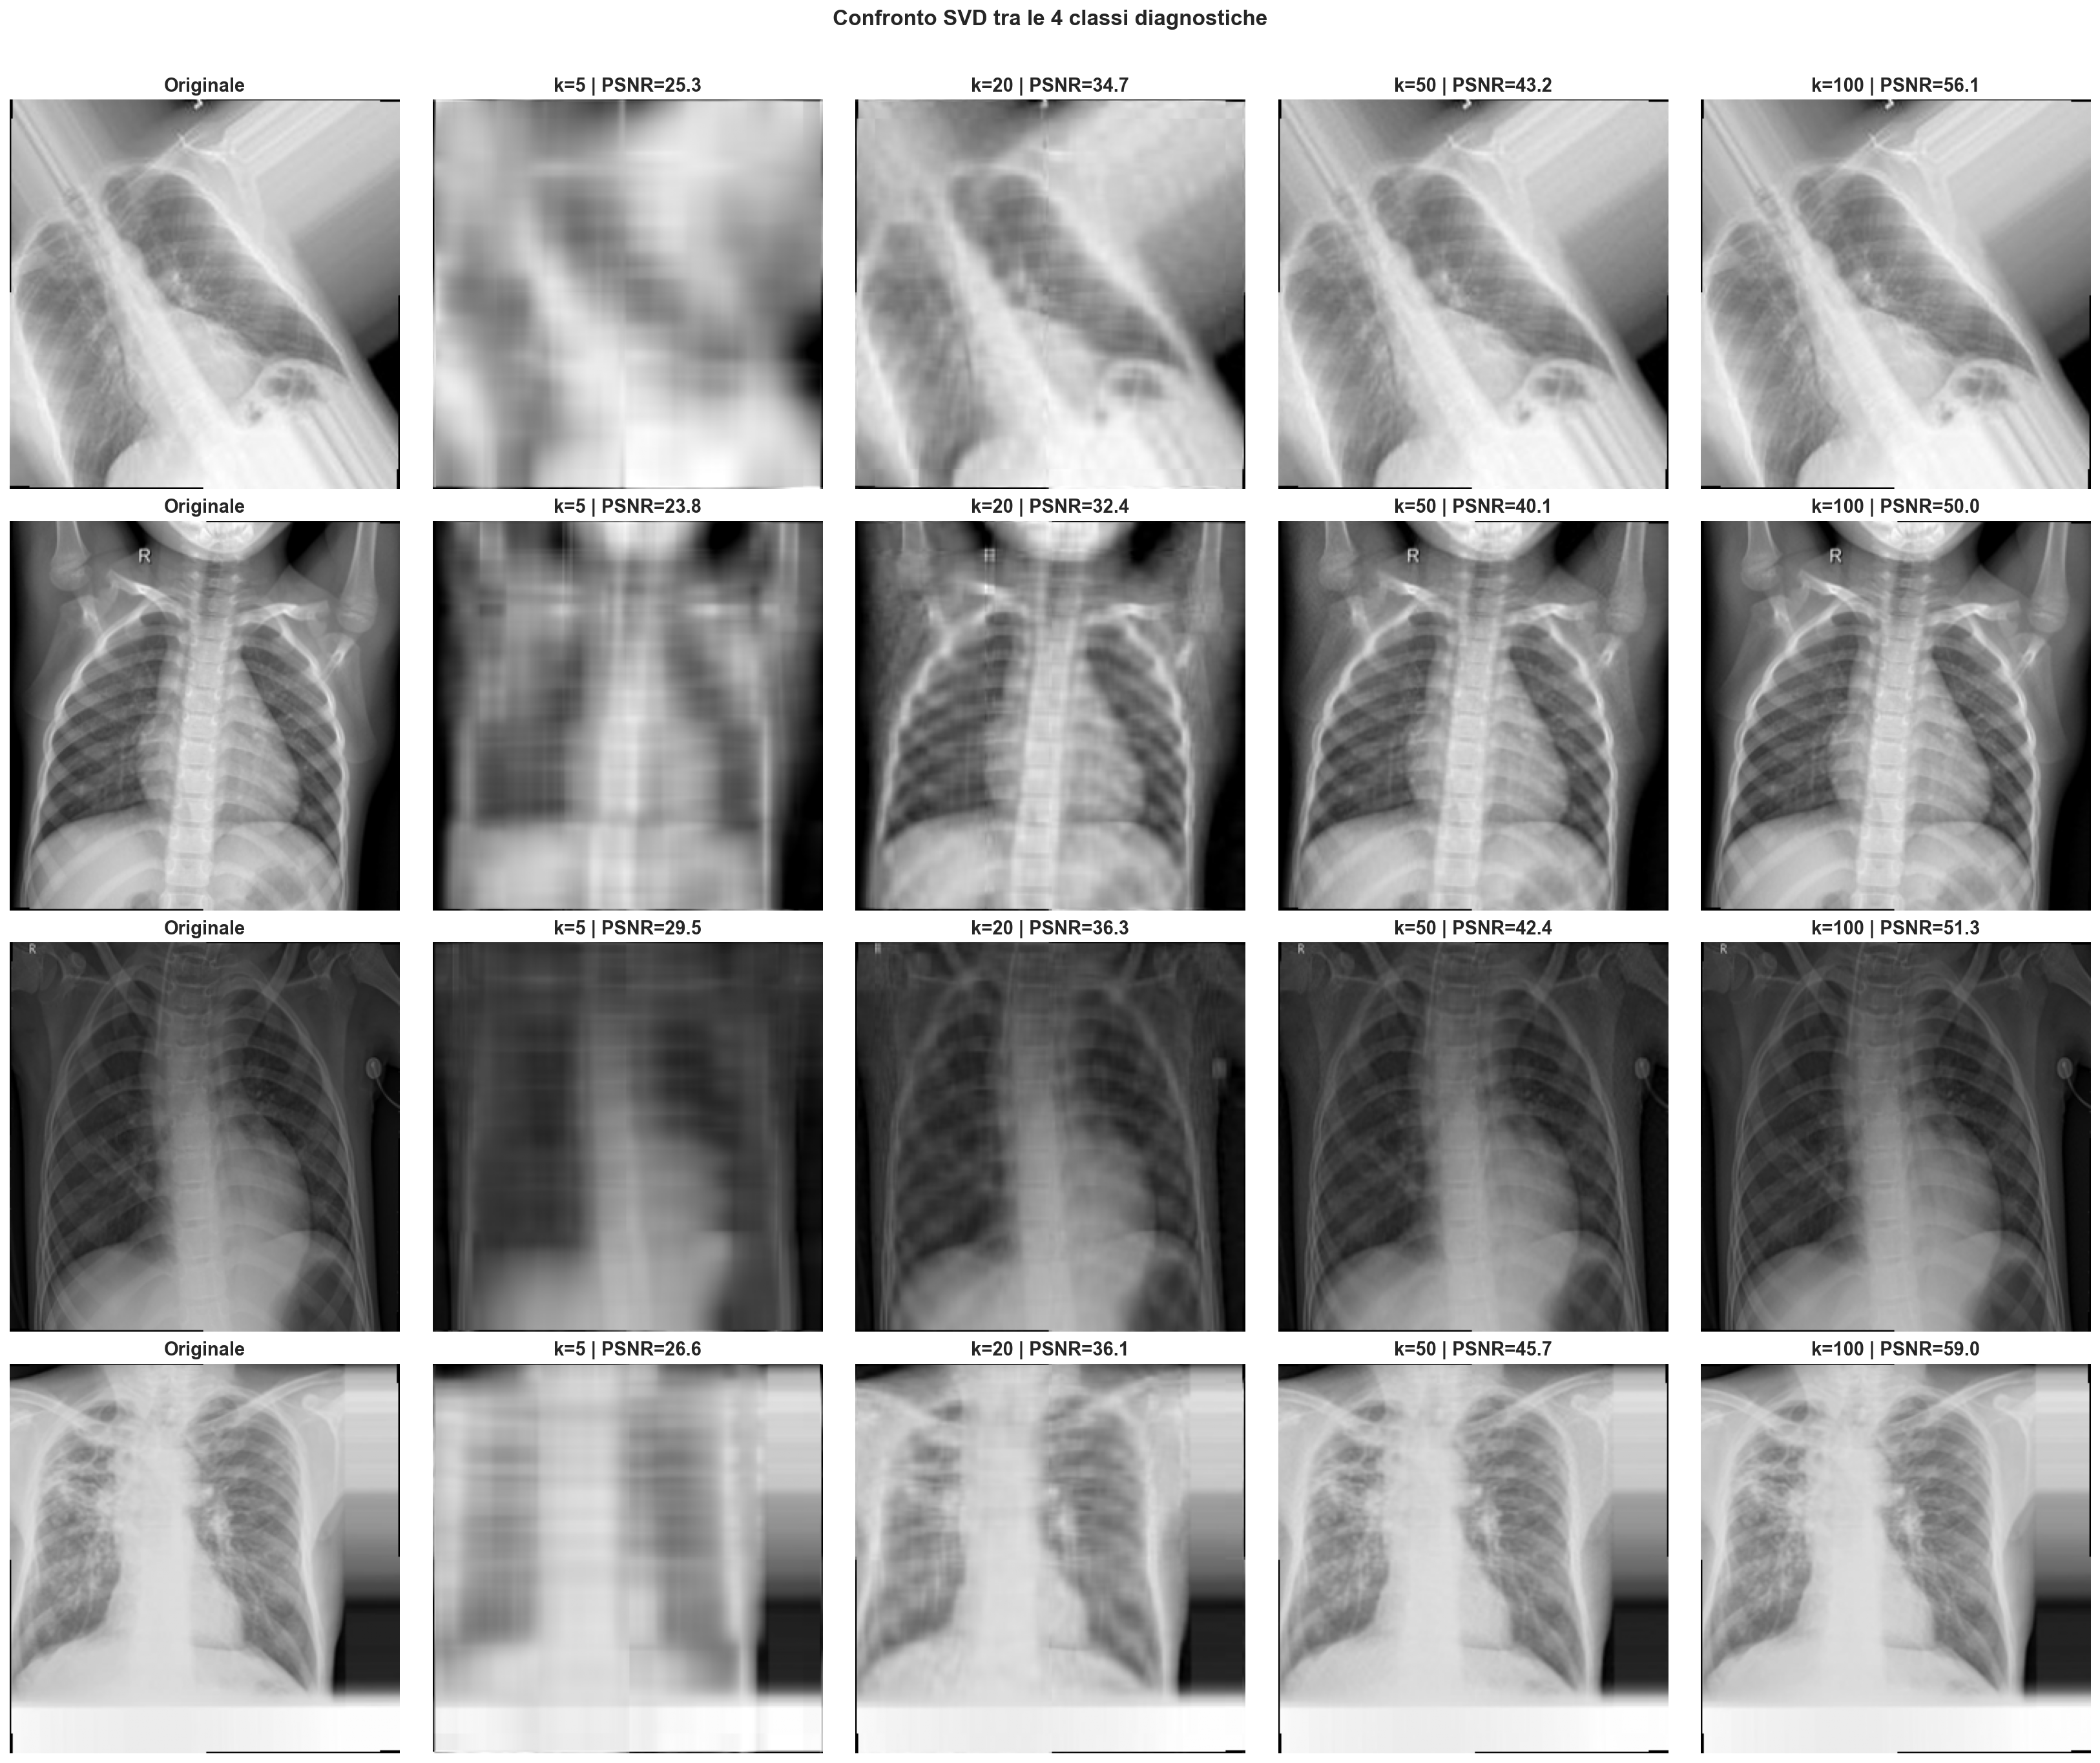
\includegraphics[width=\linewidth]{fase4_confronto_classi.png}
  \caption{Phase 4 --- SVD reconstruction comparison across the four classes
           at $k \in \{5, 20, 50, 100\}$.}
\end{figure}

All four classes reach PSNR $> 30$ dB at $k = 20$ and PSNR $> 48$ dB at
$k = 100$. Pneumonia and Tuberculosis achieve slightly higher PSNR at the same
$k$, indicating lower-rank structure (more compressible). COVID-19 and Normal
show marginally higher MSE at low $k$, consistent with their greater structural
complexity.

\subsection{Phase 5 --- Statistical Analysis and PCA}

\subsubsection{Scree Plot and Singular Value Decay}

\begin{figure}[H]
  \centering
  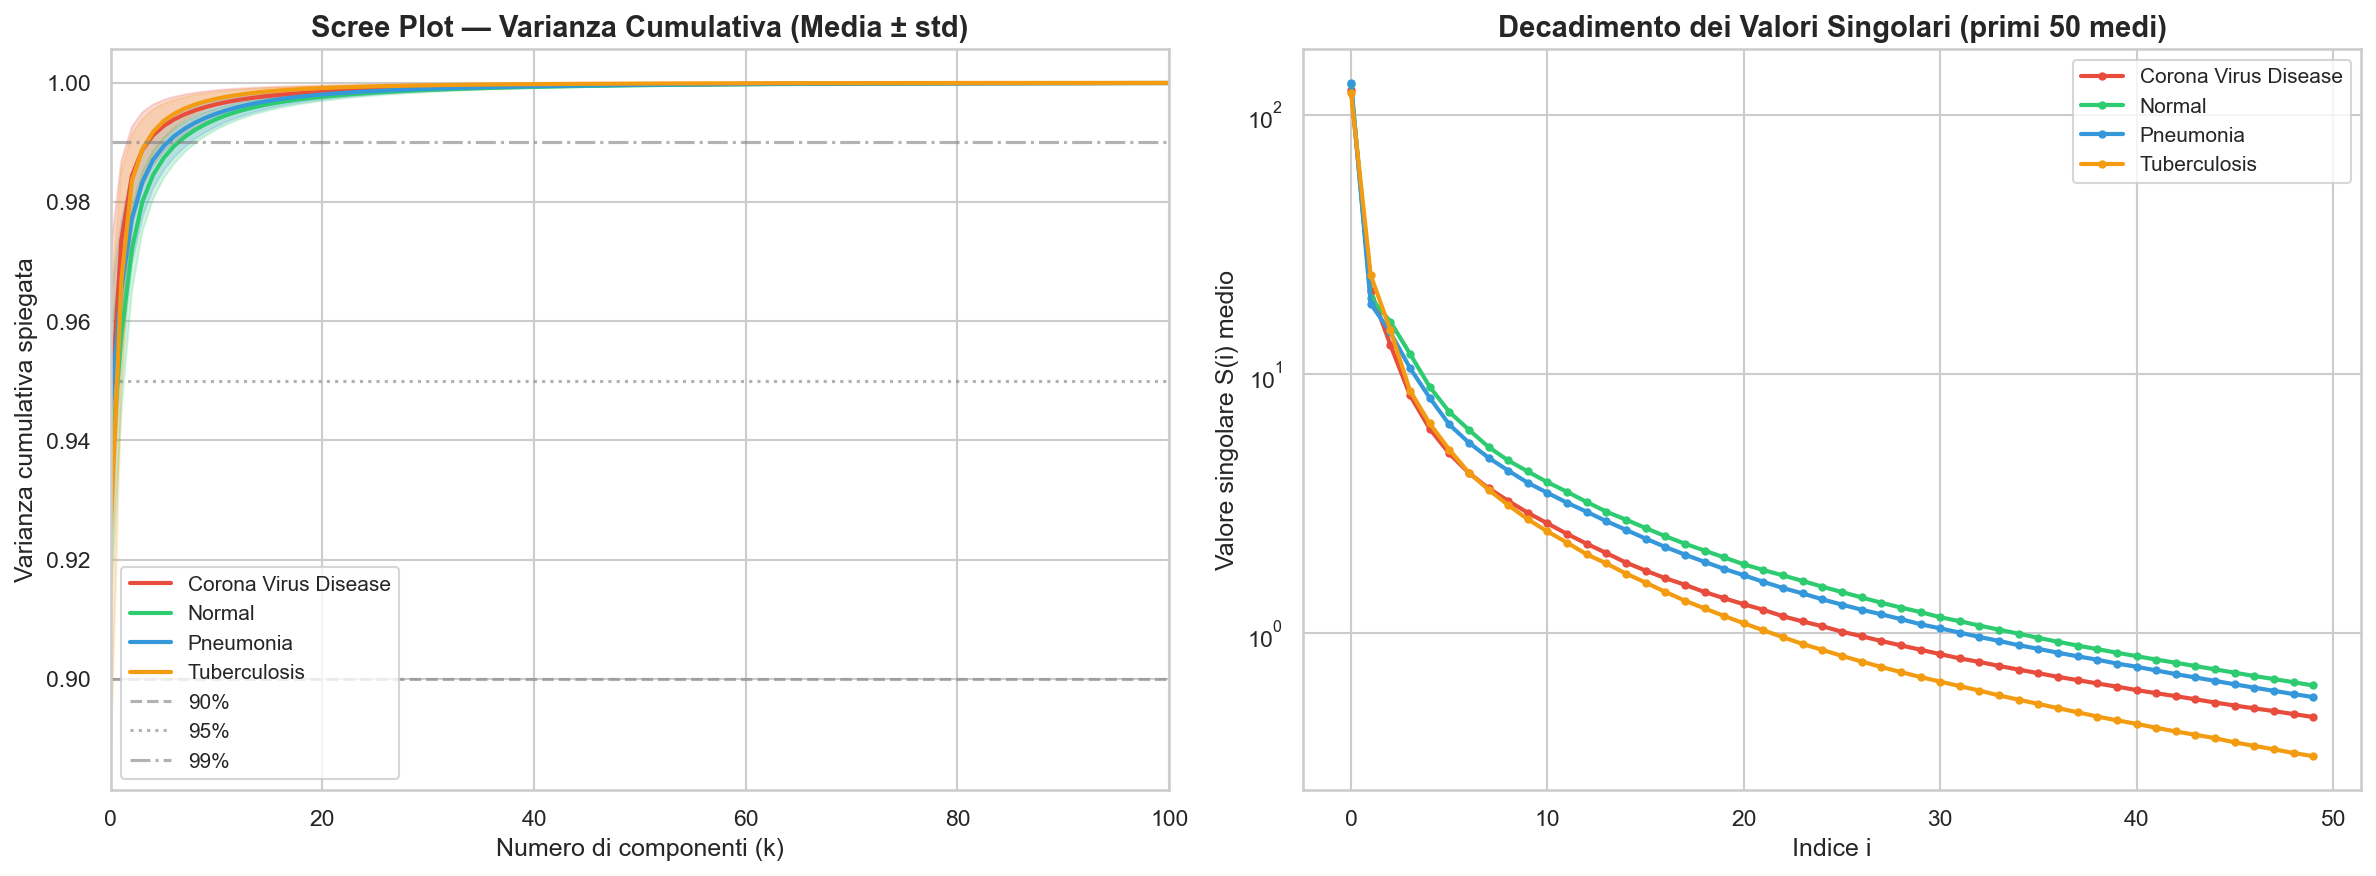
\includegraphics[width=\linewidth]{fase5_scree_plot.png}
  \caption{Phase 5 --- Cumulative variance explained (left) and singular value
           decay (right, log scale) for each class.}
\end{figure}

\begin{table}[H]
\centering
\begin{tabular}{lrrrr}
\toprule
\textbf{Class} & $k_{90\%}$ & $k_{95\%}$ & $k_{99\%}$ & Total\\
\midrule
COVID-19     & $\approx$1--3 & $\approx$5--10 & $\approx$20--40 & 256 \\
Normal       & $\approx$1--3 & $\approx$5--10 & $\approx$20--40 & 256 \\
Pneumonia    & $\approx$1--3 & $\approx$5--10 & $\approx$20--40 & 256 \\
Tuberculosis & $\approx$1--3 & $\approx$5--10 & $\approx$20--40 & 256 \\
\bottomrule
\end{tabular}
\caption{Minimum $k$ required to reach each variance threshold.
         Results are consistent across all classes.}
\end{table}

\noindent All classes exhibit a \textbf{strong low-rank structure}: 90\% of the
image energy is concentrated in only 1--3 singular components. This is a direct
consequence of the high spatial correlation in chest radiographs (uniform
background, repeated curved rib structures).

\subsubsection{MSE and PSNR Curves vs. $k$}

\begin{figure}[H]
  \centering
  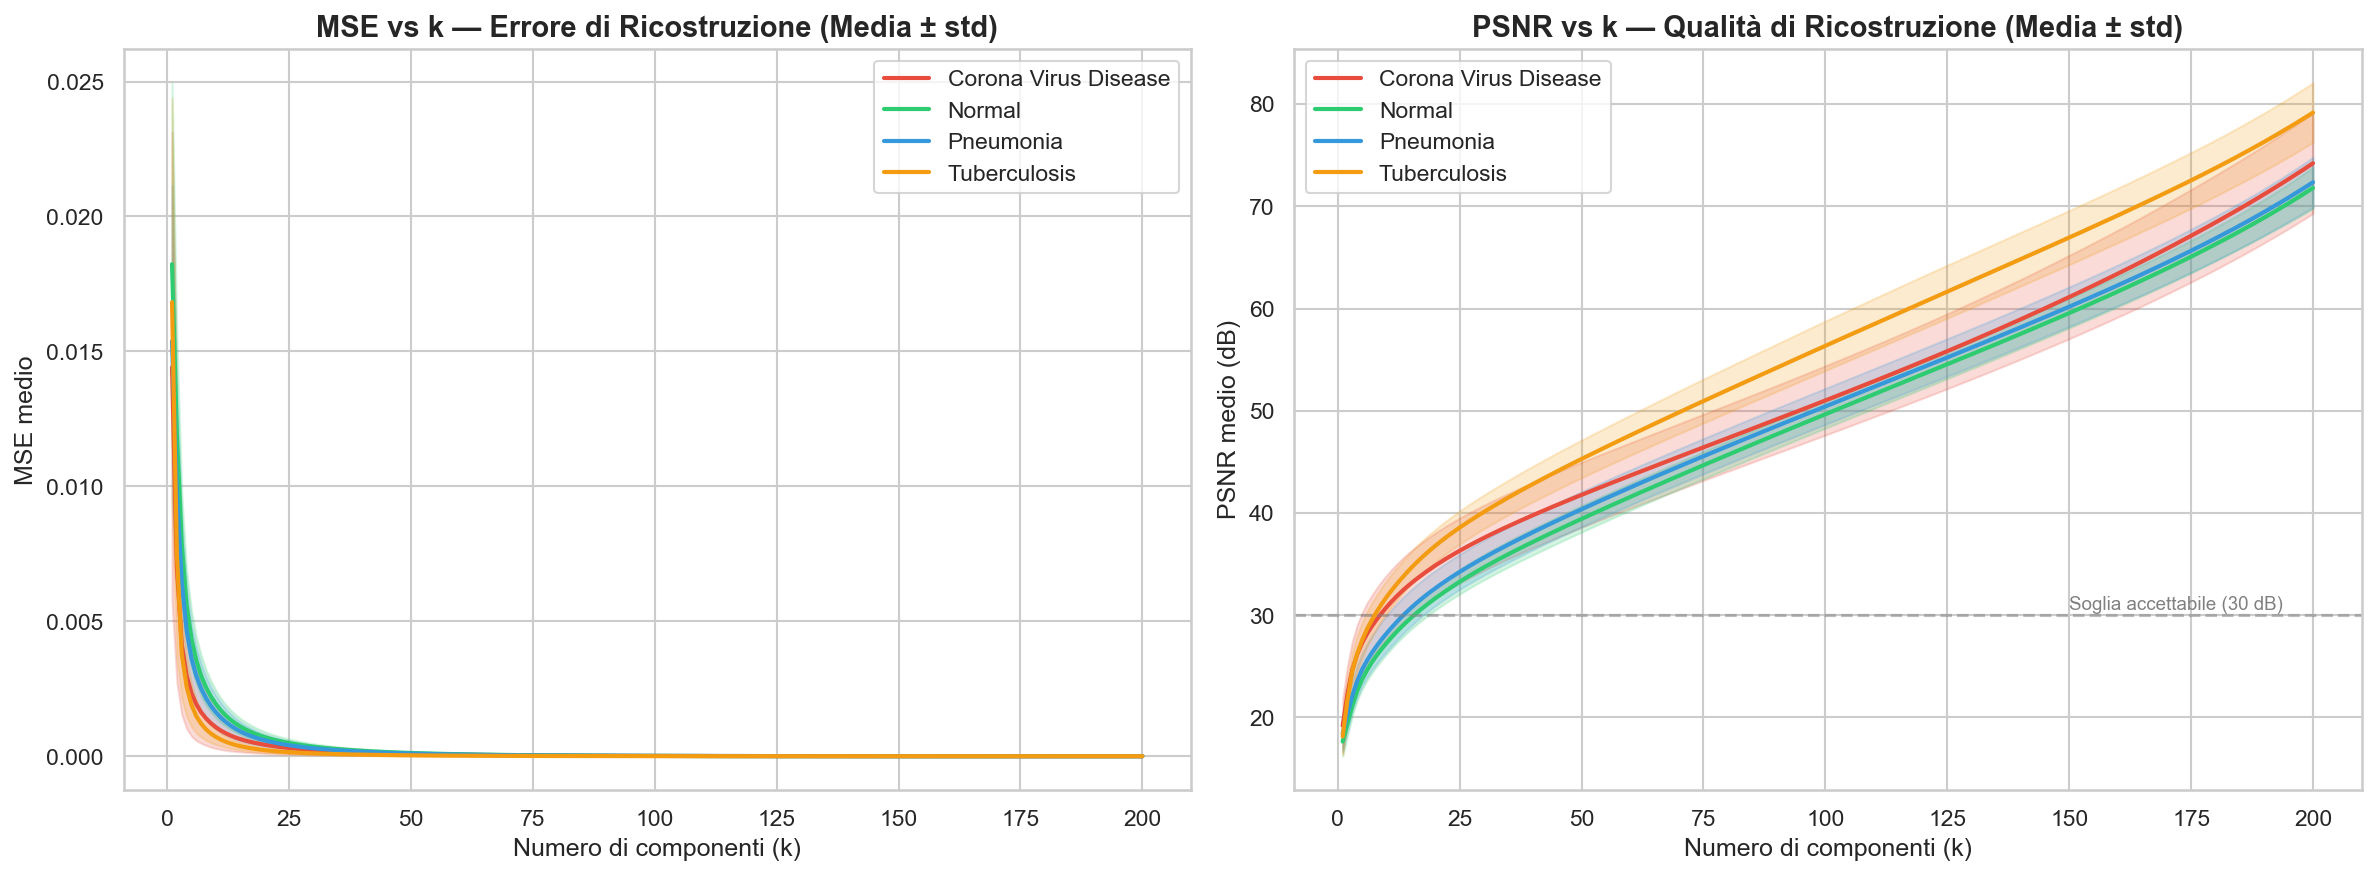
\includegraphics[width=\linewidth]{fase5_mse_psnr.png}
  \caption{Phase 5 --- MSE (left) and PSNR (right) as a function of $k$ for each class.}
\end{figure}

\begin{itemize}[nosep]
  \item \textbf{MSE} decays rapidly up to $k \approx 20$--30, then stabilises.
  \item \textbf{PSNR} grows logarithmically; the ``elbow'' (maximum marginal gain) is at $k \approx 20$--50.
  \item COVID-19 and Normal show slightly higher MSE at low $k$, confirming
        their greater structural complexity.
\end{itemize}

\subsubsection{PCA --- 2D Projection and Class Separability}

\begin{figure}[H]
  \centering
  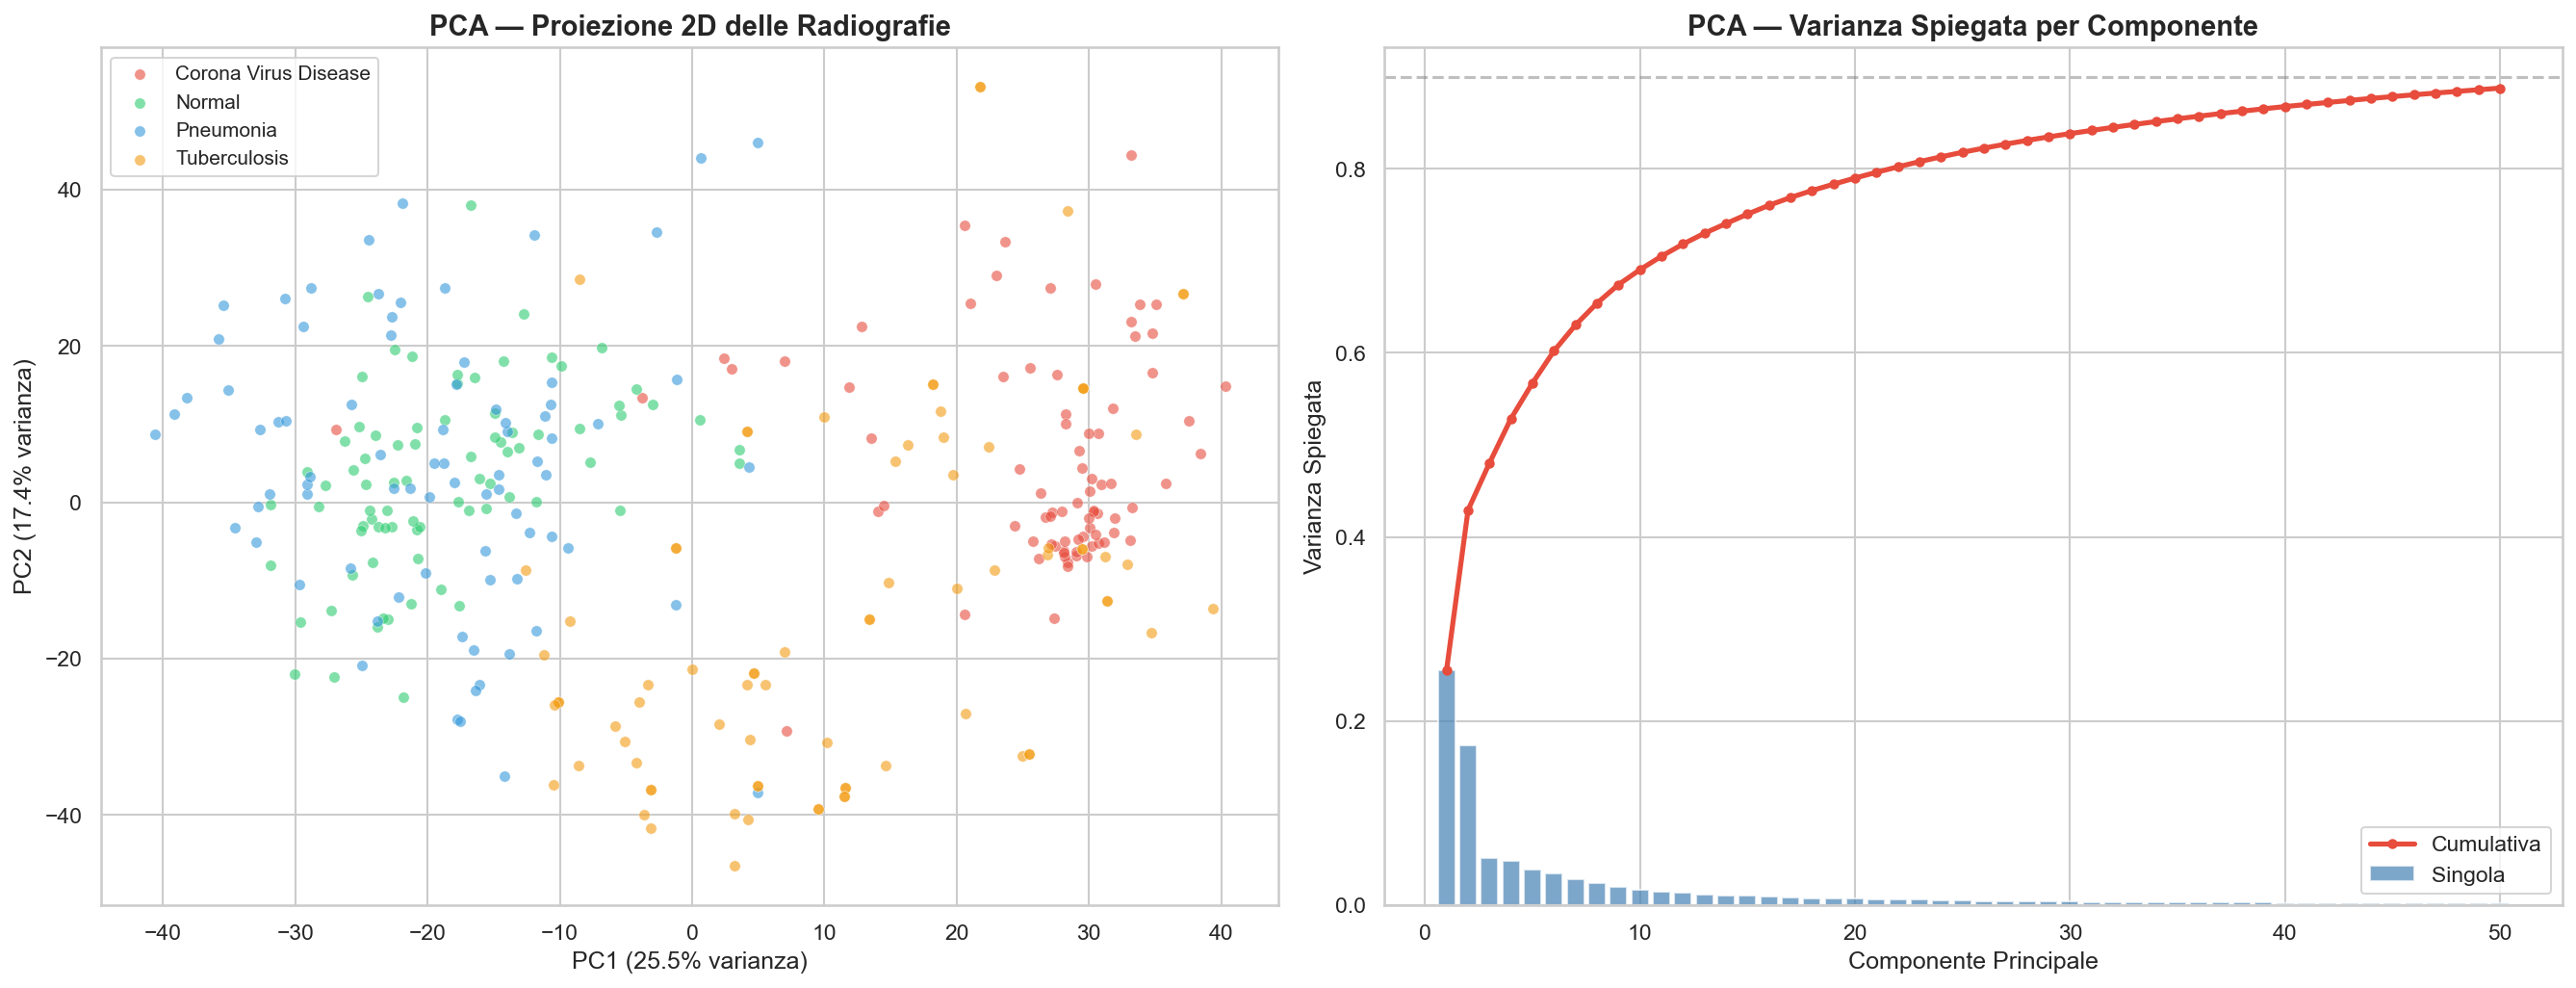
\includegraphics[width=\linewidth]{fase5_pca_scatter.png}
  \caption{Phase 5 --- PCA scatter plot (left) and per-component explained
           variance (right). The first 50 components explain $\approx 90\%$ of the total variance.}
\end{figure}

\noindent\textbf{Results:}
\begin{itemize}[nosep]
  \item PC1 (25.6\% variance) and PC2 (17.4\%) together explain \textbf{43\%} of total variance.
  \item \textbf{Normal} and \textbf{Pneumonia} cluster on the left (PC1 $< 0$);
        \textbf{COVID-19} and \textbf{Tuberculosis} on the right (PC1 $> 0$).
  \item Considerable class \textbf{overlap} remains --- partial but not perfect separability.
\end{itemize}

\subsubsection{Eigen-X-rays}

\begin{figure}[H]
  \centering
  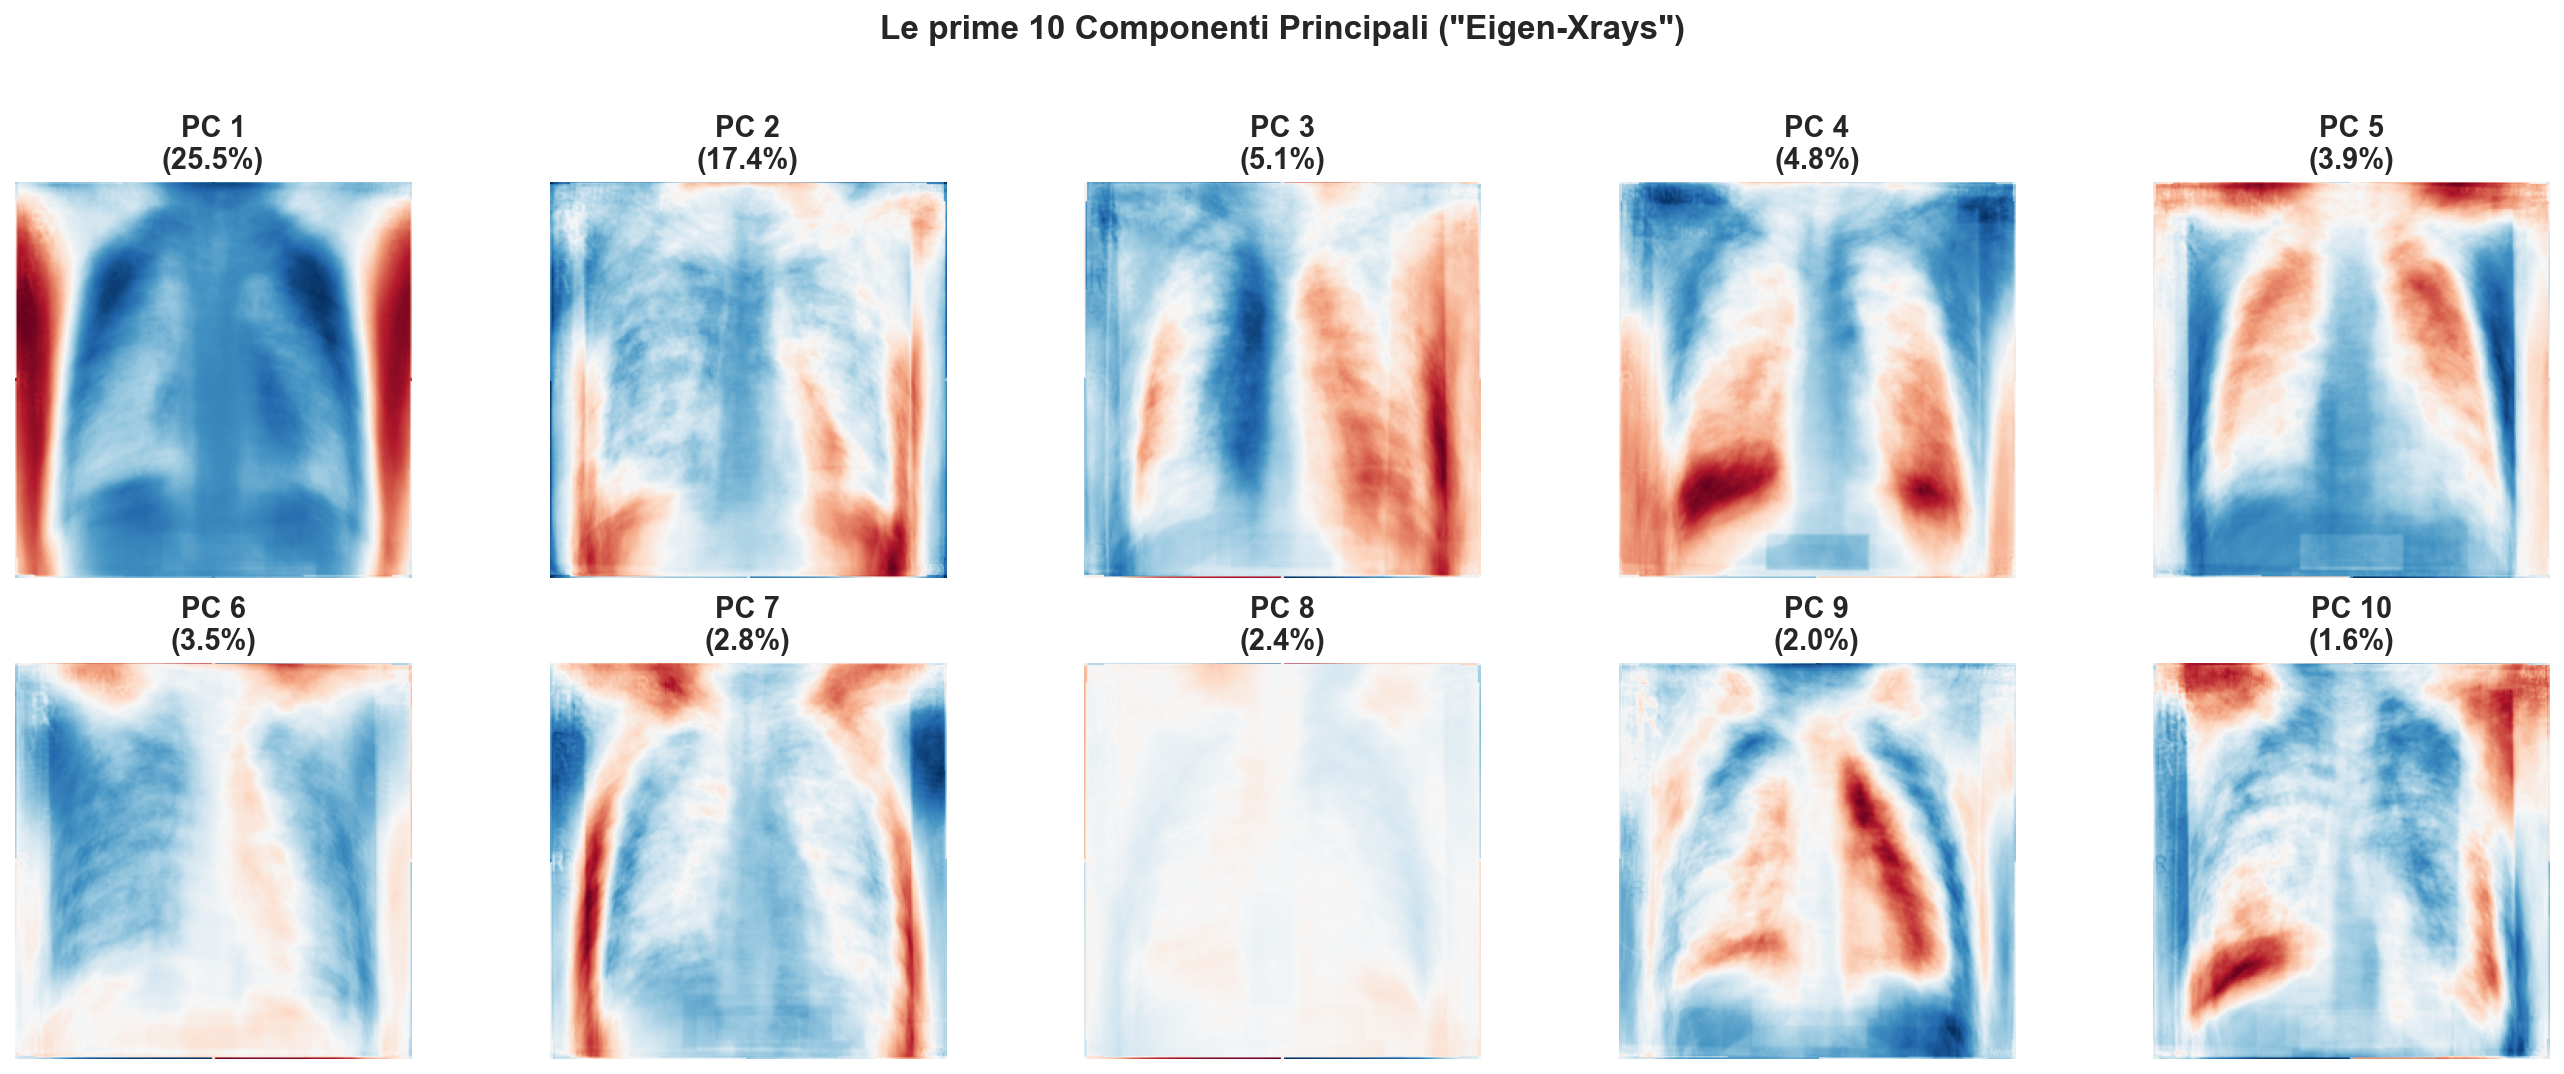
\includegraphics[width=\linewidth]{fase5_eigenfaces.png}
  \caption{Phase 5 --- The first 10 principal components visualised as
           $256\times 256$ images (RdBu colormap). Red = positive contribution;
           blue = negative contribution.}
\end{figure}

\begin{table}[H]
\centering
\begin{tabular}{clp{7cm}}
\toprule
\textbf{Component} & \textbf{Variance} & \textbf{Clinical interpretation} \\
\midrule
PC1  & 25.6\% & Global brightness contrast --- separates bright from dark X-rays \\
PC2  & 17.4\% & Lateral thoracic symmetry --- left vs.\ right lung profile \\
PC3  & 5.1\%  & Mediastinal pattern --- central zone variations \\
PC4  & 4.8\%  & Rib cage structures --- costal grid pattern \\
PC5--10 & 1.6--3.9\% & Fine details: lung fields, diaphragm, apices \\
\bottomrule
\end{tabular}
\caption{Clinical interpretation of the first 10 principal components.}
\end{table}


% ═══════════════════════════════ SECTION 5 ═══════════════════════════════════
\section{Comments and Analysis of Results}

\subsection{SVD for Compression --- Key Findings}

The Eckart--Young theorem guarantees theoretical optimality; the experiments
confirm it empirically. The critical operating point is $k = 20$:
\begin{itemize}[nosep]
  \item \textbf{Compression ratio:} $15.7\%$ --- only $\sim$1/6 of the original data.
  \item \textbf{PSNR:} 32.4 dB --- above the conventional 30 dB diagnostic threshold.
  \item \textbf{Behaviour is class-agnostic:} all four pathologies reach acceptable quality at the same $k$.
\end{itemize}

\subsection{PCA for Exploratory Analysis --- Key Findings}

\begin{enumerate}[nosep]
  \item \textbf{Low-rank structure is universal.} 90\% of image variance is encoded by 1--3 singular values across all classes, regardless of pathology. This reflects the high spatial correlation inherent to chest radiographs.
  \item \textbf{Eigen-X-rays reveal clinically interpretable patterns.} The algorithm ``discovers'' global contrast (PC1), bilateral symmetry (PC2), and mediastinal structure (PC3) purely from data --- without any anatomical prior.
  \item \textbf{Partial class separability exists.} The COVID-19/Tuberculosis group is separated from Normal/Pneumonia along PC1, but intra-group overlap remains. PCA alone is insufficient for reliable diagnosis.
\end{enumerate}

\subsection{Limitations}

\begin{description}[nosep, leftmargin=2em]
  \item[Imbalanced dataset.] Normal dominates the class distribution ($\times4$ vs.\ COVID-19), potentially biasing PCA components.
  \item[Heterogeneous resolution.] Aggressive downscaling (e.g., $1678 \to 256$ px for Normal) discards fine detail that may be diagnostically relevant.
  \item[Pixel-wise metrics.] MSE and PSNR do not measure perceptual or clinical quality directly.
  \item[Single-image SVD.] The SVD analysis characterises one sample per class; variability within a class is not captured.
  \item[Unsupervised PCA.] PCA maximises global variance, not inter-class discriminability. Supervised alternatives (LDA, kernel PCA) may yield better separation.
\end{description}

\subsection{Answers to the Research Questions}

\begin{enumerate}
  \item \textbf{Can SVD compress chest X-rays without diagnostic loss?} \\
    \textbf{Yes.} At $k=20$ (15.7\% storage), PSNR $> 32$ dB. At $k=50$ (39.1\%), PSNR $> 40$ dB. The Eckart--Young theorem guarantees this is the best possible rank-$k$ approximation.

  \item \textbf{Can PCA distinguish pulmonary pathologies?} \\
    \textbf{Partially.} The projection onto PC1--PC2 separates COVID-19/Tuberculosis from Normal/Pneumonia, but with significant overlap. SVD and PCA are powerful \emph{exploratory} tools that support --- but do not replace --- supervised classifiers for clinical diagnosis.
\end{enumerate}

\subsection{Possible Extensions}

\begin{itemize}[nosep]
  \item \textbf{JPEG comparison.} At equal compression ratio, is SVD competitive with the cosine-based JPEG standard?
  \item \textbf{Spatial error map.} Visualise where reconstruction error concentrates anatomically (background vs.\ lesion regions).
  \item \textbf{t-SNE.} Non-linear dimensionality reduction may reveal sharper inter-class boundaries.
  \item \textbf{Supervised reduction.} Linear Discriminant Analysis (LDA) directly maximises class separability.
\end{itemize}

% ═══════════════════════════════ CONCLUSION ══════════════════════════════════
\section*{Conclusions}

\begin{table}[H]
\centering
\begin{tabularx}{\linewidth}{lX}
\toprule
\textbf{Result} & \textbf{Evidence} \\
\midrule
SVD compresses X-rays effectively & $k=20$ (15.7\% data) $\Rightarrow$ PSNR $>32$ dB \\
Radiographs have strong low-rank structure & 90\% variance in $k\approx 1$--3 components \\
Eckart--Young guarantees optimality & No rank-$k$ method can do better \\
PCA $\equiv$ SVD on centred data & Same mathematical foundation, complementary goals \\
Eigen-X-rays reveal clinical patterns & PC1: contrast, PC2: symmetry, PC3: mediastinum \\
Partial class separability via PCA & COVID-19/TB vs.\ Normal/Pneumonia separated on PC1 \\
Pre-processing is critical & Tilt correction and image filtering improve PCA quality \\
\bottomrule
\end{tabularx}
\end{table}

% ═══════════════════════════════════════════════════════════════════════════════
\end{document}
